%
We now showcase CST using its k-NN implementation (k-NN CST).
Throughout this section, we compare it to its standard counterpart (k-NN ST) of \textcite{Thanh_KnnSituationTesting2011} and counterfactual fairness (CF) of \textcite{Kusner2017CF}.
Henceforth, we drop the ``k-NN'' for CST and ST. 
As noted in Remark~\ref{rem:SearchCenters}, we exclude the search centers when comparing CST to ST (i.e., CST w/o) and include them (i.e., CST w/) when comparing CST to CF.\footnote{The code is available in this repository: \href{https://github.com/cc-jalvarez/counterfactual-situation-testing}{https://github.com/cc-jalvarez/counterfactual-situation-testing}.}

\subsection{Setup}
\label{sec:Experiments.SetUp}

We use a significance level of $\alpha=0.05$, an accepted deviation of $\tau=0.0$, and the neighborhood sizes of $k \in \{ 15, 30, 50, 100, 250 \}$. In practice, we expect these parameters to be provided by the legal context. For instance, $k=30$ is a common size used in non-algorithmic situation testing \parencite{Rorive2009_ProvingDiscrimination}. See Appendix~\ref{Appendix.AddExperiments} for additional experiments.

Section~\ref{sec:Experiments.IllustrativeExample} focuses on comparing CST to ST and CF, while Section~\ref{sec:Experiments.Real} focuses on illustrating CST for multidimensional discrimination testing.
We use synthetic and real data, each describing high-stakes decision-making scenarios involving an ADM $b()$.
We assume a corresponding SCM $\mathcal{M}$ and DAG $\mathcal{G}$ for each scenario.
$\mathcal{M}$ and $\mathcal{G}$ are only needed for CST and CF.
Similar to $\alpha$, $\tau$, and $k$, we expect $\mathcal{M}$ and $\mathcal{G}$ to be provided.
% For $\mathcal{M}$, we assume additive noise. It is a convenient but not a necessary assumption that simplifies the abduction step when generating $\mathcal{D}^{CF}$. It implies $\mathcal{S} = \{W_j \leftarrow f_j(W_{pa(j)}) + U_j \}_{j=1}^p$ in \eqref{eq:SCM}.
The assumptions on $\mathcal{M}$ and $\mathcal{G}$ in Section~\ref{sec:CausalKnowledge} simplify the abduction step when generating $\mathcal{D}^{CF}$. We stress that these assumptions are convenient but not necessary.

\subsection{An Illustrative Example}
\label{sec:Experiments.IllustrativeExample}

%
\begin{figure}[t]
    \centering
    \begin{subfigure}{.45\linewidth}
    \includegraphics[scale=0.45]{figures/Histogram_X1.png}
    \end{subfigure}
    \hfill
    \begin{subfigure}{.45\linewidth}
    \includegraphics[scale=0.45]{figures/Histogram_X2.png}
    \end{subfigure}
\caption{Distribution of the attributes used by the ADM $b()$ in Section~\ref{sec:Experiments.IllustrativeExample}. The histograms compare the $\mathcal{D}$ and $\mathcal{D}^{CF}$ datasets for the female applicants. The shift to the right of both $X_1^{CF}$ and $X_2^{CF}$ shows the negative impact of $A$ on $X_1$ and $X_2$.}
\label{fig:LoanApp_Distributions}
\end{figure}
%

Let us consider the loan application scenario introduced in Example~\ref{ex:IllustrativeExample}.
We create the synthetic dataset $\mathcal{D}$ based on Figure~\ref{fig:KarimiV2}. 
It is a modified version of~\textcite[Figure 1]{Karimi2021_AlgoRecourse}. 
We add the protected attribute gender ($A$), which affects an applicant's annual salary ($X_1$) and bank balance ($X_2$) used by the bank's ADM $b()$ for approving ($\widehat{Y}=1$) or rejecting ($\widehat{Y}=0$) a loan application.
%
We generate $\mathcal{D}$ for $n=5000$ under $A \sim \text{Ber}(0.45)$ with $A=1$ if the individual is female and $A=0$ otherwise.
We define $f_1$ as $X_1 \leftarrow (-\$1500) \cdot \text{Poi}(10) \cdot A + U_1$ and $f_2$ as $X_2 \leftarrow (-\$300) \cdot \mathcal{X}^2(4) \cdot A + (3/10) \cdot X_1 + U_2$, assuming $U_1 \sim \$10000 \cdot \text{Poi}(10)$ and $U_2 \sim \$2500 \cdot \mathcal{N}(0, 1)$.
We define $b()$ as $\widehat{Y} = \mathbbm{1}\{ X_1 + 5 \cdot X_2 > \$225000\}$.
%
Importantly,
with Figure~\ref{fig:KarimiV2} we have access to the data generating model of $\mathcal{D}$.
It allows to study CST when we are able to control for potential model misspecifications in the SCM $\mathcal{M}$. 
$\mathcal{D}$ represents a biased scenario in which female applicants are penalized systematically in $X_1$ and $X_2$. Such penalties, e.g.,~capture the financial burdens female professionals face in the present after having been discouraged in the past from pursuing high-paying, male-oriented jobs \parencite{CriadoPerez2019InvisibleWomen}.
$\mathcal{D}$ represents a non-neutral status quo and, thus, a setting of interest to indirect non-discrimination law \parencite{Wachter2020BiasPreserving}.

We study the behavior of $b()$ toward $A$ in $\mathcal{D}$.
We use CST, ST, and CF to answer whether $b()$ discriminates against female loan applicants.
For CST and CF, we generate $\mathcal{D}^{CF}$ using Figure~\ref{fig:KarimiV2} based on the intervention $do(A:=0)$, or \textit{what would have happened had all loan applicants been male}? 
Comparing $\mathcal{D}$ to $\mathcal{D}^{CF}$ already highlights the unwanted systematic effects of $A$. 
These effects can be seen in Figure~\ref{fig:LoanApp_Distributions} by the rightward shift experienced in $X_1$ and $X_2$ for all female applicants when going from the factual to the counterfactual world.
$\mathcal{D}$ has a total of 1712 females (34.29\%) and, overall, $b()$ has an acceptance rate of 53.5\%.
Using \textit{demographic parity} (DP) \parencite{Kamiran2009_ClassifyingWihtoutDiscriminating}, we also observe the unfairness of $b()$ with 13.5\% acceptance probability for female and 40\% for male applicants.\footnote{\label{foot:dp}Formally, we define DP as $P(\hat{Y}|A=1) = P(\hat{Y}|A=0)$. We only use DP as we do not have access to the ground-truth $Y$ and cannot use, e.g.,~equalized odds \parencite{DBLP:conf/nips/HardtPNS16}.}

Table~\ref{table:k-results} reports the results for all methods based on Definitions~\ref{def:IndDisc} and \ref{def:CIs}.
Under Definition~\ref{def:IndDisc}, we detect individual discrimination when the complainant's $\Delta p > \tau$; and under Definition~\ref{def:CIs}, we detect individual discrimination that is statistically significant given $\alpha$ when $\Delta p > \tau$ and $\tau$ does not fall within $\Delta p$'s CI.
Figures~\ref{fig:CSTwoVsST_k_param}
% , \ref{fig:CSTwiVsCF_k_param}, 
and \ref{fig:TwoCSTs_k_param} further show how the results change under these definitions for all methods as $k$ increases, including cases beyond $k=250$.
Let us discuss these results in detail.

%
\begin{table}[t]
\caption{Number and (\% w.r.t. females) of individual discrimination cases based on $A$ in Figure~\ref{fig:KarimiV2}. Marked by * are the number of statistically significant cases.}
  \label{table:k-results}
  \centering
  \begin{tabular}{cccccc}
    \toprule
    Method & $k=15$ & $k=30$ & $k=50$ & $k=100$ & $k=250$\\
    \midrule
    CST w/o & 288 (16.8\%) & 313 (18.3\%) & 342 (20\%) & 395 (23.1\%)  & 534 (31.2\%) \\
     & 272* (15.9\%) & 306* (17.9\%) & 331* (19.3\%) & 383* (22.4\%)  & 519* (30.3\%) \\
     \midrule
    ST & 55 (3.2\%) & 65 (3.8\%) & 84 (5\%) & 107 (6.3\%) & 204 (11.9\%) \\
    & 44* (2.6\%) & 57* (3.3\%) & 65* (3.8\%) & 85* (5\%) & 148 (8.6\%) \\
    \midrule
    CST w/ & 420 (24.5\%) & 434 (25.4\%) & 453 (26.5\%) & 480 (28\%)  & 557 (32.5\%)\\
    & 272* (15.9\%) & 307* (17.9\%) & 334* (19.5\%) & 385* (22.5\%)  & 520 (30.4\%)\\
    \midrule
    CF &  376 (22\%) &  376 (22\%) &  376 (22\%) & 376 (22\%)  & 376 (22\%) \\
    & 241* (14.1\%) &  253* (14.8\%) & 265* (15.5\%) & 288* (16.8\%)  & 352* (20.6\%) \\
    \bottomrule
  \end{tabular}
\end{table}
%

\subsubsection{CST Relative to ST}
\label{sec:Experiments.IllustrativeExample.CSTvST}

We consider CST w/o as ST excludes the search centers when testing for individual discrimination. What is clear from Table~\ref{table:k-results} is that CST w/o detects more cases than ST across all $k$ sizes, even when accounting for statistical significance. The results highlight the impact of operationalizing \textit{fairness given the difference} since the only difference between the two methods is the choice of the test search center. 
ST performs an idealized comparison. If we consider the tuple $(x_1=35000, x_2=7948, a=1)$ as complainant $c$, then ST builds the test group by finding the $k$ most similar male profiles under $d$ \eqref{eq:Distance} using $c$ as the test search center. CST w/o, conversely, performs a more flexible comparison under \textit{fairness given the difference}. For the same $c$ and $d$ \eqref{eq:Distance}, it instead uses the counterfactual tuple $(x_1^{CF}=50796, x_2^{CF}=13852, a^{CF}=0)$ as the test search center. The control group is the same for both ST and CST as each uses $c$ as the control search center.

Figure~\ref{fig:LoanApp_BoxPlots} shows the impact of \textit{fairness given the difference}.
We randomly choose five complainants that are discriminated by $b()$ according to ST and CST w/o for $k=15$, and plot the distributions of $X_1$ and $X_2$ as boxplots for the control group (ctr), ST test group (tst-st), and CST w/o test group (tst-cf).
The tst-cf are above the tst-st boxplots, indicating male profiles that are likelier to be accepted by $b()$. 
As all 55 ST cases for $k=15$ are included in the 288 CST w/o cases, the difference in test groups explains the difference in the number of cases between the methods.
Tables~\ref{table:k-results_for_STandCST} and \ref{table:k-results_for_CSTnotinST} illustrate this point.

%
\begin{table}[t]
\caption{Summary statistics for cases detected by ST and CST w/o for $k=15$. We present the averages for the control groups (ctr's) and the corresponding test groups (tst's).}
  \label{table:k-results_for_STandCST}
  \centering
  \begin{tabular}{cccc}
    \toprule
    Average of & ctr's for ST and CST w/o & tst's for ST & tst's for CST w/o \\
    \midrule
    Num. of neg. $\hat{Y}$ & 8.82 & 2.22 & 0.00 \\
    Prp. of neg. $\hat{Y}$ & 0.59 & 0.15 & 0.00 \\
    Avg. Annual salary & 94372.12 & 96181.82 & 106569.70 \\
    Std. Annual salary & 1646.29 & 611.57 & 286.34 \\
    Avg. Account balance & 26092.93 & 26347.46 & 30141.28 \\
    Std. Account balance & 558.30 & 352.78 & 273.45 \\
    \bottomrule
  \end{tabular}
\end{table}
%

%
\begin{table}[t]
\caption{Summary statistics, similar to Table~\ref{table:k-results_for_STandCST} but for all cases detected by CST w/o only. We include the corresponding ST test groups for comparison.}
  \label{table:k-results_for_CSTnotinST}
  \centering
  \begin{tabular}{cccc}
    \toprule
    Average of & ctr's for ST and CST w/o & tst's for ST & tst's for CST w/o \\
    \midrule
    Num. of neg. $\hat{Y}$ & 13.74 & 14.79 & 0.78 \\
    Prp. of neg. $\hat{Y}$ & 0.92 & 0.99 & 0.05 \\
    Avg. Annual salary & 86332.47 & 85911.30 & 96898.43 \\
    Std. Annual salary & 1524.33 & 906.11 & 391.49 \\
    Avg. Account balance & 24734.11 & 24790.05 & 28677.11 \\
    Std. Account balance & 482.15 & 152.07 & 171.61 \\
    \bottomrule
  \end{tabular}
\end{table}
%

Table~\ref{table:k-results_for_STandCST} reports the average summary statistics for the cases detected by ST and CST w/o for $k=15$.
Notice that (the average of) the average and standard deviation for $X_1$ and $X_2$ are similar between the ST control and test groups, while such similarity does not occur between the CST w/o groups.
The CST w/o test groups show a higher annual salary and account balance than their ST counterparts. 
It translates into a lower average number and proportion of negative $\hat{Y}$ as these male profiles are likelier to be accepted by $b()$.
There is still a clear difference in outcomes between the control groups and the ST and CST w/o test groups, which leads to both methods detecting these cases.
% \footnote{ We exclude the distance to the search centers in Tables \ref{table:k-results_for_STandCST} and \ref{table:k-results_for_CSTnotinST} as these are similar for ST and CST w/o groups. The distance minimized by the k-NN is group-specific. Group composition is more informative.}

Table~\ref{table:k-results_for_CSTnotinST} reports the same summary statistics but for cases detected by CST w/o only. 
For comparison, we include the corresponding ST test groups. 
The groups for ST are again similar (and lower in average values) between them in terms of $X_1$ and $X_2$, but are also similar in terms of the number of negative $\hat{Y}$, explaining why ST does not detect these cases. 
The CST w/o test groups, instead, exhibit almost no cases of negative $\hat{Y}$. 
Intuitively, 
ST is comparing females and males with similar applicants not suitable for a loan while CST w/o is comparing non-suitable female to suitable male applicants.
This difference between ST and CST w/o is stark because $\mathcal{D}$ is purposely generated with a systematic bias against female applicants. 
We expect the CST w/o test groups to be more suitable than their ST counterparts as the former's test search centers account for the downstream effects of $A$ on $X_1$ and $X_2$ while the latter's test search centers ignore any effect at all.

Figure~\ref{fig:CSTwoVsST_k_param} illustrates how CST w/o and ST differ in terms of number of discrimination cases and $\Delta p$ up until $k=500$ for all and statistically significant cases.
In both plots, CST w/o and ST follow a similar trend and with signs of a slow convergence toward the other.
The impact of the \textit{mutatis mutandis} over the \textit{ceteris paribus} manipulation occurs on smaller $k$'s and persists over larger $k$'s, clearly differentiating CST w/o from ST and its operationalization of \textit{fairness given the difference} for sensible ranges of $k$.
The higher number of cases by CST w/o over ST (left) is driven by test groups that are, on average, dissimilar to the control groups, leading to a larger average $\Delta p$ by CST w/o over ST (center).
Both methods show similar trends when considering all and statistically significant cases, meaning the difference between CST w/o and ST is statistically significant.
The results validate the use of CST w/o over ST as well as the viability of the \textit{mutatis mutandis} over the \textit{ceteris paribus} manipulation for testing discrimination.

%
\begin{figure}[t]
    \centering
    \begin{subfigure}{.45\linewidth}
    \includegraphics[scale=0.45]{figures/STvsCST_X1.png}
    \end{subfigure}
    \hfill
    \begin{subfigure}{.45\linewidth}
    \includegraphics[scale=0.45]{figures/STvsCST_X2.png}
    \end{subfigure}
\caption{The boxplots for a subset of cases detected by ST and CST w/o for $k=15$. We compare the ST and CST w/o control group (ctr) versus the ST (tst-st) and CST w/o (tst-cf) test groups. 
%
The tst-st are closer to ctr than tst-cf, illustrating the \textit{fairness given the difference} behind CST and the \textit{idealized comparison} behind ST.}
\label{fig:LoanApp_BoxPlots}
\end{figure}
%

%
\begin{figure}[t]
    \centering
    \begin{subfigure}{.32\linewidth}
    \includegraphics[scale=0.345]{figures/CSTwoVsST_nums_versus_k.png}
    \end{subfigure}
    \hfill
    \begin{subfigure}{.32\linewidth}
    \includegraphics[scale=0.345]{figures/CSTwoVsST_delta_versus_k.png}
    \end{subfigure}
    \hfill
    \begin{subfigure}{.32\linewidth}
    \includegraphics[scale=0.345]{figures/CSTwiVsCF_nums_versus_k.png}
    \end{subfigure}
\caption{Left and center: Number of cases by CST w/o and ST and their avg. $\Delta p$. Right: Number of cases by CST w/ and CF. We plot all and statistically significant (sig.) cases.}
\label{fig:CSTwoVsST_k_param}
\label{fig:CSTwiVsCF_k_param}
\end{figure}
%

\subsubsection{CST Relative to CF}
\label{sec:Experiments.IllustrativeExample.CSTvCF}

We consider the CST w/ as CF uses the search centers for measuring the counterfactual fairness of $b()$.
Back to the illustrative factual and counterfactual tuples of $c$, we now include the control search center $(x_1=35000, x_2=7948, a=1)$ and the test search center $(x_1^{CF}=50796, x_2^{CF}=13852, a^{CF}=0)$ into the k-NN neighborhoods to be compared for $c$. 
These are the two instances we compare under CF to test for the counterfactual fairness of $b()$.
For comparison, we define CF discrimination as a case in which the factual $\widehat{y}_c=0 \in \mathcal{D}$ (from negative outcome) becomes $\widehat{y}_c^{CF}=1 \in \mathcal{D}^{CF}$ (to positive outcome) after the intervention on $A$.
This definition aligns with using $\tau=0.0$ for CST w/.

% %
% \begin{figure}[t]
%     \centering
%     % \begin{subfigure}{.45\linewidth}
%     \includegraphics[scale=0.485]{figures/CSTwiVsCF_nums_versus_k.png}
%     % \end{subfigure}
%     % \hfill
%     % \begin{subfigure}{.45\linewidth}
%     % \includegraphics[scale=0.485]{figures/CSTwoVsST_delta_versus_k.png}
%     % \end{subfigure}
% \caption{Number of cases detected by CST w/ and CF. We plot all and statistically significant (sig.) cases.}
% \label{fig:CSTwiVsCF_k_param}
% \end{figure}
% %

Table~\ref{table:k-results} shows how CST w/ detects for each $k$ a higher number of cases than CF, even when accounting for statistical significance.
In fact, all cases detected by CF are also detected by CST w/.
CF is independent from $k$ as it applies only to the individual comparison of the factual and counterfactual tuples for a given $c$.
However, the CI used for measuring the statistical significance of CF discrimination is a function $k$ and, thus, varies with it (cfr.,~\eqref{eq:CIs} and \eqref{eq:CIsforCF}).
As $k$ increases, so does the number of statistically significant CF and CST w/ individual discrimination cases.
Both CST w/ and CF use the one-sided CI \eqref{eq:CIs} as we test for $\Delta p > \tau$.
%
Figure~\ref{fig:CSTwiVsCF_k_param} (right) further shows how CST w/ and CF evolve as $k$ increases up to $k=500$ in terms of the number of cases detected.
% , accounting also for those that are statistically significant.
It aligns with Table~\ref{table:k-results}. 
% Unlike Figures~\ref{fig:CSTwoVsST_k_param} and \ref{fig:TwoCSTs_k_param}, 
We do not plot the average $\Delta p$ as CF discrimination focuses on the literal comparison of the factual and counterfactual instances of $c$.
Further, the number of significant CF cases is bounded by all CF cases. 
As long as CST w/ detects more cases than CF, it appears that all CF cases become statistically significant under a large enough $k$. 

What sets CST w/ apart from CF is twofold.
%
First, CST w/ equips the CF comparison with certainty measures.
Table~\ref{table:CFwithCIs} shows individual cases of discrimination detected by both CF and CST w/ for $k=15$ along with the one-sided \eqref{eq:CIs} and two-sided \eqref{eq:CIsforCF} CI.
The latter CI is specific to CF and it is built through the CST w/ k-NN implementation. 
Beyond the CF discrimination claim, this CI provides a measure of certainty to the factual versus counterfactual comparison behind CF.
Hence, CST complements CF beyond detecting discrimination.
%
Second, CST w/ detects cases of individual discrimination that are counterfactually fair. 
In Table~\ref{table:NotinCFwithCIs} reports cases for $k=15$ that do not exhibit CF discrimination but exhibit a discriminatory pattern when looking at $\Delta p$.
The results highlight the importance of requiring multiple comparisons to insure that the complainant's experience is representative of the discrimination claim.

%
\begin{table}[t]
  \caption{Subset of cases detected by both CST w/ and CF for $k=15$. The * denotes statistical significance based on the one-sided CI.}
  \label{table:CFwithCIs}
  \centering
  \begin{tabular}{cccccc}
    \toprule
    Comp. (ID) & $p_c$ & $p_t$ & $\Delta p$ & CI \eqref{eq:CIs} & CI \eqref{eq:CIsforCF} \\
    \midrule
    44  & 1.00 & 0.00 & 1.00* & [1.00, +$\infty$) & [1.00, 1.00] \\
    55  & 0.81 & 0.00 & 0.81* & [0.65, +$\infty$) & [0.62, 1.00] \\
    150 & 1.00 & 0.94 & 0.06 & [-0.04, +$\infty$) & [-0.06, 0.18] \\
    203 & 1.00 & 0.87 & 0.13 & [-0.01, +$\infty$) & [-0.04, 0.29] \\
    218 & 0.56 & 0.00 & 0.56* & [0.36, +$\infty$) & [0.32, 0.81] \\
    \bottomrule
  \end{tabular}
\end{table}
%

%
\begin{table}[t]
  \caption{Subset of cases detected by CST w/ and not CF for $k=15$. The * denotes statistical significance based on the one-sided CI.}
  \label{table:NotinCFwithCIs}
  \centering
  \begin{tabular}{cccccc}
    \toprule
    Comp. (ID) & $p_c$ & $p_t$ & $\Delta p$ & CI \eqref{eq:CIs} & CI \eqref{eq:CIsforCF} \\
    \midrule
    5 & 0.06 & 0.00 & 0.06 & [-0.04, +$\infty$) & [-0.06, 0.18] \\
    147  & 0.50 & 0.00 & 0.5* & [0.29, +$\infty$) & [0.26, 0.75] \\
    435  & 0.38 & 0.00 & 0.38* & [0.18, +$\infty$) & [0.14, 0.61] \\
    1958 & 0.13 & 0.00 & 0.13 & [-0.01, +$\infty$) & [-0.04, 0.29] \\
    2926 & 0.75 & 0.00 & 0.75* & [0.57, +$\infty$) & [0.54, 0.96] \\
    \bottomrule
  \end{tabular}
\end{table}
%

Tables~\ref{table:k-results_for_CFvsCST_InBoth} and \ref{table:k-results_for_CFvsCST_InCSTOnly} report how a counterfactually fair $b()$ still discriminates according to CST w/.
As argued in Section~\ref{sec:CST.OnCF}, it occurs when considering a complainant and its counterfactual that are close to and on the same side of the decision boundary of $b()$.
When building the neighborhoods, CST w/ may include profiles from both sides of the decision boundary.
Table~\ref{table:k-results_for_CFvsCST_InBoth} summarizes the group characteristics of the cases detected by CF and CST w/.
If we consider (the average of) the average $X_1$ and $X_2$ for control and test groups, we obtain that $b()$ rejects the former and accept the latter, meaning it is not counterfactually fair.
Table~\ref{table:k-results_for_CFvsCST_InCSTOnly}, instead, summarizes cases detected by CST w/. 
For those cases, using again (the average of) the average $X_1$ and $X_2$ for control and test groups, $b()$ accepts both.
% : i.e., $b()$ is counterfactually fair. 

%
\begin{table}[t]
\caption{Summary statistics for cases detected by both CF and CST w/ under $k=15$. We present averages for the control groups (ctr’s) and the test groups (tst’s).}
  \label{table:k-results_for_CFvsCST_InBoth}
  \centering
  \begin{tabular}{ccc}
    \toprule
    Average of & ctr's CST w/ & tst's for CST w/ \\
    \midrule
    Num. of neg. $\hat{Y}$ & 15.46 & 5.75 \\
    Prp. of neg. $\hat{Y}$ & 1.03 & 0.38 \\
    % Avg. $d$ to search center & 0.03 & 0.04 & 0.03 \\
    Avg. Annual salary & 83281.25 & 94323.46 \\
    Std. Annual salary & 1410.97 & 1564.37 \\
    Avg. Account balance & 23752.64 & 27762.60 \\
    Std. Account balance & 449.85 & 550.18 \\
    \bottomrule
  \end{tabular}
\end{table}
%
%
\begin{table}[t]
\caption{Summary statistics for cases detected by CST w/ under $k=15$ and not CF. We present averages for the control groups (ctr’s) and the test groups (tst’s).}
  \label{table:k-results_for_CFvsCST_InCSTOnly}
  \centering
  \begin{tabular}{ccc}
    \toprule
    Average of & ctr's CST w/ & tst's for CST w/ \\
    \midrule
    Num. of neg. $\hat{Y}$ & 5.23 & 0.00 \\
    Prp. of neg. $\hat{Y}$ & 0.35 & 0.00 \\
    % Avg. $d$ to search center & 0.03 & 0.04 & 0.03 \\
    Avg. Annual salary & 92892.05 & 104541.25 \\
    Std. Annual salary & 1592.33 & 1434.18 \\
    Avg. Account balance & 26890.63 & 31161.38 \\
    Std. Account balance & 509.61 & 545.73 \\
    \bottomrule
  \end{tabular}
\end{table}
%

\subsubsection{CST w/o and CST w/}
\label{sec:Experiments.IllustrativeExample.BothCST}

Finally, we consider the two CST versions.
Three patterns are clear in Table~\ref{table:k-results}.
First, CST w/ detects a higher number of individual discrimination cases than CST w/o for all $k$.
Second, this difference decreases between the CST versions as $k$ increases.
Third, CST w/ and CST w/o detect roughly the same number of cases when accounting for statistical significance.
Let us explore these patterns.
Note that $\tau = 0.0$; any deviation of $p_c$ from $p_t$ (read, $\Delta p$) is detected by CST. 
Such deviation is statistically significant (read, representative) depending on the composition of the control and test groups behind $p_c$ and $p_t$. 

What differentiates CST w/o from w/ is the exclusion of the search centers (Remark~\ref{rem:SearchCenters}), making the size of the neighborhoods under CST w/o of size $k$ and under CST w/ of size $k+1$. 
Back to the illustrative factual and counterfactual tuples of $c$, the CST w/o control and test group are the same as the CST w/ ones with the key difference that the CST w/ control group has a \textit{(k+1)-th} that is $(x_1=35000, x_2=7948, a=1)$ and the test group has a \textit{(k+1)-th} that is $(x_1^{CF}=50796, x_2^{CF}=13852, a^{CF}=0)$.
The additional tuple pair compared in CST w/ is, notably, the most important pair
% : the complainant and its counterfactual.
% This is the ``most important pair'' 
as the complainant and its counterfactual denote the closest possible comparison under CST.
Clearly, the inclusion (or exclusion) of the complainant-counterfactual pair into $\Delta p$ of CST w/ (or CST w/o) drives the statistically insignificant difference in the number of detected cases. 
Based on Table~\ref{table:k-results}, such pair is able to deviate $\Delta p$ from $\tau$ but is not representative of the corresponding control and test neighborhoods. 

%
\begin{table}[t]
\caption{Summary statistics for CST w/o cases for $k=15$ for the control (ctr’s) and test groups (tst’s) split by statical significance, which we denote with *.}
  \label{table:CST_without_k15}
  \centering
  \begin{tabular}{ccccc}
    \toprule
    Average of & ctr's & tst's & ctr's* & tst's* \\
    \midrule
    Num. of neg. $\hat{Y}$ & 3.94 & 2.62 & 13.32 & 0.51 \\
    Prp. of neg. $\hat{Y}$ & 0.26 & 0.17 & 0.89 & 0.03 \\
    Avg. Annual salary & 92808.34 & 104750.00 & 87577.21 & 98392.16 \\
    Std. Annual salary & 1919.18 & 1182.73 & 1525.77 & 323.69 \\
    Avg. Account balance & 25923.28 & 30121.55 & 24938.92 & 28888.21 \\
    Std. Account balance & 652.67 & 290.97 & 487.52 & 185.18 \\
    \bottomrule
  \end{tabular}
\end{table}
%

%
\begin{table}[t]
\caption{Summary statistics for CST w/ cases for $k=15$ for the control (ctr’s) and test groups (tst’s) split by statical significance, which we denote with *.}
  \label{table:CST_with_k15}
  \centering
  \begin{tabular}{ccccc}
    \toprule
    Average of & ctr's & tst's & ctr's* & tst's* \\
    \midrule
    Num. of neg. $\hat{Y}$ & 14.72 & 13.66 & 14.21 & 0.51 \\
    Prp. of neg. $\hat{Y}$ & 0.92 & 0.86 & 0.89 & 0.03 \\
    Avg. Annual salary & 78240.29 & 89308.43 & 87578.81 & 98705.10 \\
    Std. Annual salary & 1331.29 & 1672.54 & 1483.66 & 1484.45 \\
    Avg. Account balance & 22503.79 & 26478.22 & 24939.78 & 29011.26 \\
    Std. Account balance & 422.47 & 554.67 & 474.41 & 547.02 \\
    \bottomrule
  \end{tabular}
\end{table}
%

Let us consider the two CST versions for $k=15$.
Tables \ref{table:CST_without_k15} and \ref{table:CST_with_k15} summarize the control and test groups, respectively, of CST w/o and CST w/ split by statistical significance.
%
These tables are not mutually exclusive as CST w/o and CST w/ detect the same 272 statistically significant cases and the 288 CST w/o cases are included in the 420 CST w/ cases in Table~\ref{table:k-results}. 
The group pairs within each table are mutually exclusive as, different from previous tables, we split between statistically significant and non-significant cases. 
%
Based on the average characteristics in both tables, these groups are almost identical and enjoy, on average, a large $\Delta p$'s. 
Together, it explains why the inclusion (exclusion) of the the complainant and its counterfactual from, respectively, the control and test group in CST w/ (CST w/o) has little impact on these cases.
%
Comparing now the significant versus non-significant control and test groups in each table, we observe that the latter have a smaller difference between the average number of negative $\hat{Y}$ per group, which explains why these cases are detected by CST w/o and w/ but do not amount to statistically significant cases.

The non-statistically significant cases in Tables \ref{table:CST_without_k15} and \ref{table:CST_with_k15} vary more than the statistically significant cases in terms of their composition, with CST w/ having a considerably larger average number of negative decisions.
This difference illustrates the role of including/excluding the search centers and their representativeness relative to their corresponding neighborhoods.
Here, recall that CST w/ almost doubles CST w/o for all cases. 
CST w/ detects cases with more heterogeneous neighborhoods in terms of applicant suitability, which would explain the lower average proportion of negative outcomes.
CST w/, instead, detects more homogeneous neighborhoods marked by a lack of suitability due to the large average proportion of negative outcomes. What occurs for the non-statistically significant CST w/ groups is that the complainant and its counterfactual disagree, meaning the former is rejected and the latter is accepted, which would be enough to deviate $\Delta p$ from $\tau$ while both control and test neighborhoods appear to be, on average, clearly non-suitable. 

%
\begin{figure}[t]
    \centering
    \begin{subfigure}{.45\linewidth}
    \includegraphics[scale=0.45]{figures/twoCST_nums_versus_k.png}
    \end{subfigure}
    \hfill
    \begin{subfigure}{.45\linewidth}
    \includegraphics[scale=0.45]{figures/twoCST_delta_versus_k.png}
    \end{subfigure}
\caption{Number of cases by CST w/o and w/ and their average $\Delta p$, respectively. We plot all and statistically significant (sig.) cases for both versions of CST.}
\label{fig:TwoCSTs_k_param}
\end{figure}
%

What about for larger neighborhood sizes? 
In Table~\ref{table:k-results}, CST w/o and CST w/ converge in number of cases as $k$ increases.
We argue that this occurs as larger neighborhoods diminish the impact of the \textit{(k+ 1)-th} pair, meaning the CST w/ is, in fact, converging toward CST w/o.
In Figure~\ref{fig:TwoCSTs_k_param} we plot the effect of increasing $k$ up to 500 on the number of discrimination cases and their average $\Delta p$. 
We do so for both CST versions, differentiating between all and statistically significant cases.
These plots align with Table~\ref{table:k-results}.
The plots support the previous analysis for Tables \ref{table:CST_without_k15} and \ref{table:CST_with_k15} regarding the impact of the additional pair in CST w/.
Consider the plots for the number of discrimination cases (left). As $k$ increases, the number of cases increases for all four. Notably, CST w/o's all and statistically significant cases and CST w/'s statistically significant cases align throughout $k$, while CST w/'s all cases converges to these three.
The same pattern occurs when we look at the plots for average $\Delta p$ (right), though the average $\Delta p$ decreases as $k$ increases.

Given Table~\ref{table:k-results} and Figure~\ref{fig:TwoCSTs_k_param}, it is worth asking whether having two versions of CST is useful?
Each version targets a different method, CST w/o relative to ST and CST w/ relative to CF; however, we might prefer CST w/o if expected to provide statistically significant results. 
% Further, in that case, we might use CST w/o also to link ST and CF.
What matters is that the difference between ST and both CST versions holds, highlighting the impact of using a \textit{mutatis mutandis} over a \textit{ceteris paribus} manipulation when testing for discrimination.
Also important is that we are able to provide certainty measures around CF under both CST versions as long as $k$ is large enough for $\Delta p$ under CST w/ to converge to $\Delta p$ under CST w/o.

Finally, the discrepancy between the CST versions raises questions on what it means for a $\Delta p$ to be representative.
Consider that we have not constrained $\mathcal{D}^{CF}$ w.r.t. $\mathcal{D}$, meaning it is possible for the counterfactual instances to deviate considerably from the factual instances. 
In that case, we would have ``unrepresentative'' counterfactual instances that motivate statistically insignificant comparisons, but that are still ``unavoidable'' in the sense that these same instances embody scenarios that should have happened for the complainants according to a SCM $\mathcal{M}$.
We believe that judging the representativeness of the counterfactual world by using the factual world as the underlying population might not properly capture the substantive equality goals behind non-discrimination law \parencite{Wachter2020BiasPreserving}. 
We come back to this last discussion in Section~\ref{sec:Discussion}.

\subsection{Law School Admissions}
\label{sec:Experiments.Real}

%
\begin{figure}[t]
\begin{minipage}{.35\linewidth}
\begin{figure}[H]
\centering
    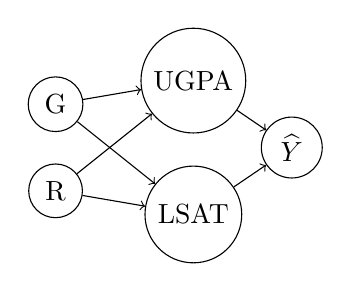
\begin{tikzpicture}
        \node (A1)  at (-1.75, -0.55) [circle, draw]{R};
        \node (A2)  at (-1.75, 0.55) [circle, draw]{G};
        \node (X1) at (0, 0.85) [circle, draw]{UGPA};
        \node (X2) at (0,-0.85) [circle,draw]{LSAT};
        \node (Y)  at (1.25, 0) [circle, draw]{$\widehat{Y}$};
        \draw[->] (A1) to (X1) {};
        \draw[->] (A1) to (X2) {};
        \draw[->] (A2) to (X1) {};
        \draw[->] (A2) to (X2) {};
        \draw[->] (X1) to (Y) {};
        % \draw[->] (X1) to (X2) {};
        \draw[->] (X2) to (Y) {};
    \end{tikzpicture}
\end{figure}
\end{minipage}
\begin{minipage}{.55\linewidth}
\begin{align*}
\mathcal{M} \, & 
\begin{cases}
    R & \leftarrow U_{R}\\
    G & \leftarrow U_G \\
    UGPA & \leftarrow b_U + \beta_1 \cdot R + \lambda_1 \cdot G + U_1, \ \\
    LSAT & \leftarrow  \exp\{b_L + \beta_2 \cdot R + \lambda_2 \cdot G + U_2\}, \\
\end{cases}
\end{align*}
\begin{align*}
    \widehat{Y} & = b(UGPA, LSAT) 
    % \\
    % & = \mathbbm{1}\{(0.6 \cdot UGPA + 0.4 \cdot LSAT) > \psi\}
\end{align*}
\end{minipage}
\caption{The auxiliary causal knowledge for Section~\ref{sec:Experiments.Real}. Let $R$ denote race, $G$ gender, \textit{LSAT} law school admissions test scores, \textit{UGPA} undergraduate grade-point average, and $\hat{Y}$ the admissions decision by $b()$.}
\label{fig:LawSchool}
% \vspace{-2ex}
\end{figure}
%

Let us now consider the law school admissions scenario popularized by \textcite[Figure 2]{Kusner2017CF}.
We use US data from the Law School Admission Council survey \parencite{Wightman1998_LawDataSource}, and recreate an admissions scenario for a top US law school. 
We consider as protected attributes an applicant's gender (\textit{G}, male/female), and race (\textit{R}, white/non-white). 
We add the ADM $b(UGPA, LSAT) = \hat{Y}$, which considers the applicant's undergraduate grade-point average (\textit{UGPA}) and law school admissions test scores (LSAT). 
If an applicant is successful, $\widehat{Y}=1$; otherwise $\widehat{Y}=0$. 
We summarize the scenario in Figure~\ref{fig:LawSchool}.
We define the ADM $b()$ using the median entry requirements for the top US law school to derive the cutoff $\psi$.\footnote{That being Yale University Law School; see \url{https://www.ilrg.com/rankings/law/index/1/asc/Accept}}
Formally, we define $b()$ as $\mathbbm{1}\{(0.6 \cdot UGPA + 0.4 \cdot LSAT) > \psi\}$.
The cutoff is the weighted sum of 60\%  in \textit{UGPA} (3.93 over 4.00), and 40\%  \textit{LSAT} (46.1 over 48), giving a total of 20.8; the maximum possible score given $b()$ is 22. 
The SCM $\mathcal{M}$ and DAG $\mathcal{G}$ follow \textcite{Kusner2017CF},
with $b_U$ and $b_L$ denoting the intercepts; $\beta_1$, $\beta_2$, $\lambda_1$, $\lambda_2$ the weights; and $U_1 \sim \mathcal{N}$ and $U_2 \sim \text{Poi}$ the probability distributions.

We study the behavior of $b()$ toward $G$ and $R$.
The dataset $\mathcal{D}$ contains $n=21790$ applicants, 43.8\% being female, 16.1\% being non-white, and 8.4\% being non-white-female.
%
Despite $b()$ being externally imposed by us for the purpose of illustrating the CST framework, under $b()$ only 0.8\% of the female applicants are successful compared to 1.5\% of the male applicants; similarly, only 0.2\% of the non-white applicants are successful compared to 2.2\% of the white applicants.
It is also the case when considering the intersectional group of non-white-females, with only 0.06\% of these applicants being admitted to law school based on $b()$ compared to the 2.25\% of white-female, non-white-male, and white-male successful applicants.
Notice that $b()$ is highly selective, with an acceptance rate of just 2.31\%, or 505 out of 21790 applicants considered.
Using DP as a fairness metric, $b()$ would still be considered unfair toward female, non-white, and non-white-female applicants.

\subsubsection{Single Discrimination}
\label{sec:Experiments.Real.Single}

%
\begin{table}[t]
\caption{Number (and \% w.r.t.~non-whites) of individual discrimination cases based on $R$ using Figure~\ref{fig:LawSchool}. Marked by * are the statistically significant cases.}
  \label{table:k-results_RACE}
  \centering
  \begin{tabular}{cccccc}
    \toprule
    Method & $k=15$ & $k=30$ & $k=50$ & $k=100$ & $k=250$\\
    \midrule
    CST w/o & 256 (7.3\%) & 309 (8.8\%) & 337 (9.6\%) & 400 (11.4\%)  & 503 (14.4\%) \\
     & 244* (6.9\%) & 301* (8.6\%) & 323* (9.2\%) & 391* (11.2\%)  & 494* (14.1\%) \\
     \midrule
    ST & 33 (0.9 \%) & 51 (1.5\%) & 61 (1.7\%) & 64 (1.8\%) & 78 (2.2\%) \\
    & 28* (0.8\%) & 28* (0.8\%) & 45* (1.3\%) & 47* (1.3\%) & 61 (1.7\%) \\
    \midrule
    CST w/ & 286 (8.2\%) & 309 (8.8\%) & 337 (9.6\%) & 400 (11.4\%)  & 503 (14.4\%)\\
    & 244* (6.9\%) & 301* (8.6\%) & 323* (9.2\%) & 391* (11.2\%)  & 494* (14.1\%) \\
    \midrule
    CF & 231 (6.6\%) & 231 (6.6\%) & 231 (6.6\%) &  231 (6.6\%) &  231 (6.6\%) \\
    & 190* (5.4\%) & 231* (6.6\%) & 231* (6.6\%) & 231* (6.6\%) & 231* (6.6\%) \\
    \bottomrule
  \end{tabular}
\end{table}
%

%
\begin{table}[t]
\caption{Number (and \% w.r.t.~females) of individual discrimination cases based on $G$ Figure~\ref{fig:LawSchool}. Marked by * are the statistically significant cases.}
  \label{table:k-results_GENDER}
  \centering
  \begin{tabular}{cccccc}
    \toprule
    Method & $k=15$ & $k=30$ & $k=50$ & $k=100$ & $k=250$\\
    \midrule
    CST w/o & 78 (0.8\%) & 120 (1.3\%) & 253 (2.7\%) & 296 (3.1\%)  & 493 (5.2\%) \\
     & 43* (0.5\%) & 88* (0.9\%) & 160* (1.7\%) & 221* (2.3\%)  & 341* (3.6\%) \\
     \midrule
    ST & 77 (0.8\%) & 101 (1.1\%) & 229 (2.4\%) & 258 (2.7\%) & 484 (5.1\%) \\
    & 57* (0.6\%) & 69* (0.7\%) & 111* (1.2\%) & 124* (1.3\%) & 366 (3.8\%) \\
    \midrule
    CST w/ & 99 (1.0\%) & 129 (1.4\%) & 267 (2.8\%) & 296 (3.1\%)  & 493 (5.2\%)\\
    & 54* (0.6\%) & 92* (0.9\%) & 160* (1.7\%) & 221* (2.3\%)  & 341* (3.6\%) \\
    \midrule
    CF & 56 (0.6\%) & 56 (0.6\%) & 56 (0.6\%) &  56 (0.6\%) &  56 (0.6\%) \\
    % & 20* (0.2\%) & 15* (0.2\%) & 30* (0.3\%) & 21* (0.2\%) & 32* (0.3\%) \\
    & 20* (0.2\%) & 15* (0.2\%) & 30* (0.3\%) & 21* (0.2\%) & 32* (0.3\%) \\
    \bottomrule
  \end{tabular}
\end{table}
%

Does $b()$ discriminate against non-white applicants? 
To answer this question using CST and CF, we generate the corresponding $\mathcal{D}^{CF}_R$ using Figure~\ref{fig:LawSchool} based in the intervention $do(R:=0)$, or \textit{what would have happened had all law school applicants been white?}
Similarly, does $b()$ discriminate against female applicants?
To answer this question using CST and CF, we generate the corresponding $\mathcal{D}^{CF}_G$ using Figure~\ref{fig:LawSchool} based in the intervention $do(G:=0)$, or \textit{what would have happened had all law school applicants been male?}
Both questions share the same $\mathcal{D}$.
Similar to Section~\ref{sec:Experiments.IllustrativeExample}, we use Definition~\ref{def:IndDisc} for detecting individual discrimination cases and Definition~\ref{def:CIs} for determining whether these cases are statistically significant.
Tables~\ref{table:k-results_RACE} and \ref{table:k-results_GENDER} show the results for all methods.
 
Tables~\ref{table:k-results_RACE} and \ref{table:k-results_GENDER} report similar patterns to those in Table~\ref{table:k-results}.
CST w/o detects a higher number of cases than ST; CST w/ detects a high number of cases than CF; and CST w/ detects a higher number than CST w/o. 
For all these patterns, though, the differences between the corresponding methods is smaller than those observed in Table~\ref{table:k-results}.
This is due to the composition of $\mathcal{D}$ and the nature of $b()$. 
Here, we work with a larger $\mathcal{D}$ (21790 versus 5000 applicants) and a more selective $b()$ (2.31\% versus 53.3\% acceptance rate).
CST w/o and CST w/ in Table~\ref{table:k-results_GENDER} converge already at larger neighborhood sizes, which does not occur in Table~\ref{table:k-results} (there is, though, a clear pattern that it occurs eventually as shown in Figure~\ref{fig:TwoCSTs_k_param}).
We also observe similar patterns once we account for statistical significance with CST w/o and CST w/ reaching the same number of cases in both tables for $k=250$.

%
\begin{figure}[t]
    \begin{subfigure}{.45\linewidth}
    \includegraphics[scale=0.45]{figures/R_all_delta_versus_k.png}
    \caption{}
     % \label{fig:a}
    \end{subfigure}
\hfill
    \begin{subfigure}{.45\linewidth}
    \includegraphics[scale=0.45]{figures/G_all_delta_versus_k.png}
    \caption{}
     % \label{fig:b}
    \end{subfigure}
\medskip
   \begin{subfigure}{.45\linewidth}
    \includegraphics[scale=0.45]{figures/R_all_nums_versus_k.png}
    \caption{}
     % \label{fig:c}
    \end{subfigure}
\hfill
    \begin{subfigure}{.45\linewidth}
    \includegraphics[scale=0.45]{figures/G_all_nums_versus_k.png}
    \caption{}
     % \label{fig:d}
    \end{subfigure}
\caption{Average $\Delta p$ and number of cases for race ($R$) and gender ($G$), respectively. We plot all and statistically significant (sig.) cases for each method.}
\label{fig:LawSchoolSingleDiscrimiantion_allmethods_k_param}
\end{figure}
%

Figure~\ref{fig:LawSchoolSingleDiscrimiantion_allmethods_k_param} supports Tables~\ref{table:k-results_RACE} and \ref{table:k-results_GENDER}, showing the average $\Delta p$ and the number of cases up to $k=500$ for all methods.\footnote{Due the size of $\mathcal{D}$, we run the methods for $k$ equals 1, 15, 30 and between 50-500 in increments of 10.} 
For the average $\Delta p$, as shown in sub-figures (a) and (b), it decreases as $k$ increases, with all methods seemingly converging to a single value.
%
% Notably, 
By observing that, as $k \rightarrow \infty$, the neighborhoods of the complainant and its counterfactual include all protected and unprotected instances, respectively, in $\mathcal{D}$, this value turns out to be the difference in DP: $P(\hat{Y}|A=1) - P(\hat{Y}|A=0)$ (cfr., footnote~\ref{foot:dp}) .
%
The average $\Delta p$ for significant cases is higher to, see ST in (a), or almost the same as, see CST w/ in (a), for all the cases.  
As $k$ increases, the control and tests groups constructed by ST, CST w/o, and CST w/ start considering new instances further away from the search centers and whatever detected initial deviation from $\tau$ dissipates slowly.
%
Similarly, as shown in sub-figures (c) and (d), the number of cases increases as $k$ increases except for CF which is independent of $k$ and its significant cases that are bounded by CF itself. 
We observe the CST versions converging, especially when accounting for statistical significance, while ST remains below both CST versions in (c) and mimics CST w/o in (d).
The number of significant cases is lower to ST in (c), or almost the same as both CST versions in (c) for all cases. 

The number of cases varies across the methods between Tables~\ref{table:k-results_RACE} and \ref{table:k-results_GENDER}. 
This is due to race and gender having different non-protected and protected search spaces.
The results are comparable, but represent separate tests for single discrimination.
Recall that non-whites represent 16.1\% while females represent 43.8\% of $\mathcal{D}$. 
It means that CST has access to a smaller search space when building the control groups for non-white complainants relative to female complainants.
Notably, in Table~\ref{table:k-results_RACE} statistically significant CF cases reach the 231 CF total cases within the $k$ values considered. 
This does not occur in Table~\ref{table:k-results_GENDER} in which the statistically significant CF cases slowly increase, though in a non-monotonically way, toward the 56 CF total cases.
Such oscillation, we believe, is due to the statistical estimator not yet reaching its asymptotic behavior.
These are, though, minor fluctuations as the number of statistically significant cases is around 0.2-0.3\%.\footnote{We use the CI \eqref{eq:CIs} from CST w/ though conditioned on CF discrimination occurring. We only detect 56 cases of CF discrimination (Table~\ref{table:k-results_GENDER}). As $k$ increases, we always look at these complainants.}
In Figure~\ref{fig:LawSchoolSingleDiscrimiantion_allmethods_k_param} we observe this non-monotonic increase for number of cases and decrease for the average $\Delta p$ of cases detected more clearly in the sub-figures (a) and (c) for race than for the sub-figures (b) and (d) for gender. 
The plots for gender are considerably less smooth than those for race. 
The composition of $\mathcal{D}$ clearly plays a role here as females represent 43.8\% and non-whites 16.1\% of the dataset, with the k-NN based methods varying more between iterations as they explore a much denser search space.

\subsubsection{Multidimensional Discrimination}
\label{sec:Experiments.Real.Multi}

We present the results for the forms of multidimensional discrimination, multiple and intersectional.
Given the focus on gender and race, the non-protected group amounts to the non-protected groups based on race and gender: i.e., white and male applicants.
As these two groups of applicants are not mutually exclusive, white-females and non-white-males are also part of the non-protected group.
This point is clearer when we consider the intersection of race and gender and focus on the protected group that is non-white-female applicants: the complementary of such group, meaning the non-protected group, includes white-female, non-white-male, and white-male applicants.

%
\begin{table}[t]
  \caption{Number (and \% w.r.t.~non-white-females) of multiple individual discrimination cases in Section~\ref{sec:Experiments.Real} for $R$ and $G$. Marked by * are the statistically significant cases.}
  \label{table:k-results_Multiple}
  \centering
  \begin{tabular}{cccccc}
    \toprule
    Method & $k=15$ & $k=30$ & $k=50$ & $k=100$ & $k=250$\\
    \midrule
    CST w/o & 8 (0.44\%) & 10 (0.55\%) & 20 (1.09\%) & 20 (1.09\%)  & 40 (2.18\%) \\
     & 4* (0.22\%) & 6* (0.33\%) & 11* (0.60\%) & 17* (0.93\%)  & 24* (1.31\%) \\
     \midrule
    ST & 5 (0.27\%) & 5 (0.27\%) & 12 (0.65\%) & 19 (1.04\%) & 24 (5.1\%) \\
    & 0* (0.0\%) & 0* (0.0\%) & 5* (0.27\%) & 5* (0.27\%)  & 15* (0.82\%) \\
    \midrule
    CST w/ & 9 (0.49\%) & 10 (0.55\%) & 21 (1.15\%) & 20 (1.09\%)  & 40 (2.18\%)\\
    & 4* (0.22\%) & 9* (0.49\%) & 11* (0.60\%) & 17* (0.93\%)  & 24* (1.31\%) \\
    \midrule
    CF & 5 (0.27\%) & 5 (0.27\%) & 5 (0.27\%) & 5 (0.27\%) & 5 (0.27\%) \\
    & 0* (0.0\%) & 3* (0.16\%) & 1* (0.05\%) & 1* (0.05\%) & 2* (0.11\%) \\
    \bottomrule
  \end{tabular}
\end{table}
%

%
\begin{table}[t]
  \caption{Number (and \% w.r.t.~non-white-females) of intersectional individual discrimination cases in Section~\ref{sec:Experiments.Real} for $R \times G$. Marked by * are the statistically significant cases.}
  \label{table:k-results_Intersectional}
  \centering
  \begin{tabular}{cccccc}
    \toprule
    Method & $k=15$ & $k=30$ & $k=50$ & $k=100$ & $k=250$\\
    \midrule
    CST w/o & 130 (7.1\%) & 138 (7.5\%) & 148 (8.1\%) & 160 (8.7\%)  & 199 (10.9\%) \\
    & 130* (7.1\%) & 138* (7.5\%) & 148* (8.1\%) & 160* (8.7\%)  & 199* (10.9\%) \\
     \midrule
    ST & 14 (0.8\%) & 14 (0.8\%) & 17 (0.9\%) & 24 (1.3\%) & 29 (1.6\%) \\
    & 14* (0.8\%) & 14* (0.8\%) & 13* (0.7\%) & 23* (1.3\%)  & 26* (1.4\%) \\
    \midrule
    CST w/ & 130 (7.1\%) & 138 (7.5\%) & 148 (8.1\%) & 160 (8.7\%)  & 199 (10.9\%) \\
    & 130* (7.1\%) & 138* (7.5\%) & 148* (8.1\%) & 160* (8.7\%)  & 199* (10.9\%) \\
    \midrule
    CF & 113 (6.2\%) & 113 (6.2\%) & 113 (6.2\%) & 113 (6.2\%) & 113 (6.2\%) \\
    & 113* (6.2\%) & 113* (6.2\%) & 113* (6.2\%) & 113* (6.2\%) & 113* (6.2\%) \\
    \bottomrule
  \end{tabular}
\end{table}
%

Following Definition~\ref{def:MultipleDisc}, we count as multiple discrimination based on race and gender when $\Delta p > \tau$ occurs separately for each of these protected attributes. 
Only those cases that are statistically significant for each protected attribute under CI \eqref{eq:CIs}---given the Bonferroni corrected $\alpha/2$---amount to statistically significant cases. 
We still rely on the generated $\mathcal{D}_R^{CF}$ and $\mathcal{D}_G^{CF}$ for the construction of the test groups and the original $\mathcal{D}$ for the construction of the control groups.
%
Does $b()$ discriminate against the none-white-female applicants as non-white \textit{and} as female applicants?
We present the results in Table~\ref{table:k-results_Multiple}. 
Figure~\ref{fig:LawSchoolMultiDiscrimination_allmethods_k_param}, as shown in sub-figures (a) and (c), further illustrates the results up to $k=500$. 
For the average $\Delta p$, we average those from cases detected separately under race and gender.

Following Definition~\ref{def:IntersectionaleDisc}, instead, we count intersectional discrimination based on race and gender when $\Delta p > \tau$ occurs for the intersection of these protected attributes. 
In practice, it means constructing the new protected attribute $R \times G$; updating $\mathcal{D}$ into $\mathcal{D}'$, such that $R \times G \in \mathcal{D}'$; and generating $\mathcal{D}'^{CF}$ given Figure~\ref{fig:LawSchool} under $do(R \times G := 0)$.
It implies a single discrimination run but under the ``new'' single attribute $R \times G$, representing the intersection of $R$ and $G$. 
Cases are statistically significant under CI \eqref{eq:CIs} based on $R \times G$.
Formally, in Figure~\ref{fig:LawSchool} we merge the $R$ and $G$ nodes into the single $R \times G$ in $\mathcal{G}$ node and do the same for the corresponding equations in $\mathcal{M}$ by interacting the dummy variables for $R$ and $G$ and re-estimating the regression weights \parencite{Wooldridge2015IntroductoryEconometrics}.
%
Does $b()$ discriminate against the none-white-female applicants?
We present the results in Table~\ref{table:k-results_Intersectional}.
Figure~\ref{fig:LawSchoolMultiDiscrimination_allmethods_k_param}, as shown in sub-figures (b) and (d), further illustrates the results up to $k=500$.

In Tables~\ref{table:k-results_Multiple} and \ref{table:k-results_Intersectional}, the three methods show similar patterns between them.
CST w/o detects more cases relative to ST (including statistically significant cases); CST w/ detects more cases than CF (including statistically significant cases); and the two CST versions converge once statistical significance is considered.
The same line of reasoning used before still applies here for understanding how CST, ST, and CF relate to each other.
The difference is that the protected group and, in turn, the non-protected group are defined by more than one protected attribute.
What is interesting in Table~\ref{table:k-results_Multiple} is that CST w/o and CST w/ converge early on for all cases, not just for those cases that are statistically significant.
We suspect these are cases that are clearly discriminatory under both race and gender, making them likely to be detected by multiple and intersectional discrimination testing.
All cases in Table~\ref{table:k-results_Intersectional} are also statistically significant for all methods.
It is due to $R \times G=1$ representing the most un-favored protected group from the combination of $R$ and $G$, which results in larger $\Delta p$'s and a complete convergence of all and statistically significant cases for all methods relative to multiple discrimination. 
Compare, e.g.,~(a) versus (b) and (c) versus (d) in Figure~\ref{fig:LawSchoolMultiDiscrimination_allmethods_k_param}. 
We discuss the last point in the next section.  

\subsubsection{On Multiple and Intersectional Discrimination}
\label{sec:Experiments.Real.Multiple_vs_Intersectional}

The results from the previous section support claims by legal scholars on the risk of not recognizing intersectional discrimination under non-discrimination law.
These claims, to the best of our knowledge, date back to \textcite{Crenshaw1989_DemarginalizingTheIntersection} and have become prominent again with the ongoing discussion around algorithmic discrimination \parencite{Xenidis2020_TunningEULaw}.
We suspect that, since multiple and intersectional discrimination share the protected group and the non-protected groups, there is a tendency to dismiss the latter as a special case of the former.
An in-depth legal discussion on the tension between multiple and intersectional discrimination is beyond this paper, but Tables~\ref{table:k-results_Multiple} and \ref{table:k-results_Intersectional} support the calls by these researchers to treat intersectional discrimination separate from multiple discrimination.

%
\begin{figure}[t]
    \begin{subfigure}{.45\linewidth}
    \includegraphics[scale=0.45]{figures/Multi_all_deltas_versus_k.png}
    \caption{}
    \end{subfigure}
\hfill
    \begin{subfigure}{.45\linewidth}
    \includegraphics[scale=0.45]{figures/Inter_all_deltas_versus_k.png}
    \caption{}
    \end{subfigure}
    \medskip
    \begin{subfigure}{.45\linewidth}
    \includegraphics[scale=0.45]{figures/Multi_all_nums_versus_k.png}
    \caption{}
     % \label{fig:c}
    \end{subfigure}
\hfill
    \begin{subfigure}{.45\linewidth}
    \includegraphics[scale=0.45]{figures/Inter_all_nums_versus_k.png}
    \caption{}
     % \label{fig:d}
    \end{subfigure}
\caption{Avg. $\Delta p$ and number of cases for multiple (left) and intersectional (right) discrimination on $R$ and $G$. We plot all and statistically significant (sig.) cases for all methods.}
\label{fig:LawSchoolMultiDiscrimination_allmethods_k_param}
\end{figure}
%

We acknowledge that, from a modeling perspective, a difference between Tables~\ref{table:k-results_Multiple} and \ref{table:k-results_Intersectional} is expected since we implement different procedures.
Under multiple discrimination we look at the intersection of two separate single discrimination testing runs, while under intersectional discrimination we look at a single discrimination run representing the intersection. 
%
The claims by legal scholars like \textcite{Crenshaw1989_DemarginalizingTheIntersection, Xenidis2020_TunningEULaw}, however, were not as apparent to us, meaning, in principle, we had no reason to expect a higher number of cases for intersectional discrimination over multiple discrimination.
%
In fact, from a probability theory perspective (read, the conjunction rule), if we had to choose a difference between the Tables~\ref{table:k-results_Multiple} and \ref{table:k-results_Intersectional}, we would have guessed the opposite, with multiple discrimination acting as an upper limit to intersectional discrimination.
Given these results, we now would add that such expectation holds from a modeling perspective if we agree that the intersection of $G$ and $R$ is not its own category. Let us discuss further.

The two modeling procedures allow to represent the case in which $R \times G$ is its own category (intersectional) and in which is just the conjunction of $R$ and $G$ (multiple).
This distinction, with legal origins as already argued \parencite{Crenshaw1989_DemarginalizingTheIntersection}, in fact materializes through the counterfactual representation of each complainant under these two discrimination testing procedures.
Under multiple discrimination, we still rely on $\mathcal{D}_R^{CF}$ and $\mathcal{D}_G^{CF}$ for running the methods separately on $R$ and $G$. 
We look at male and non-white conterfactuals separately. 
Although together they cover all the non-protected groups, they do not do so simultaneously: the complainant under this procedure would have been male or non-white, but not female-non-white.
%
Under intersectional discrimination, instead, we rely on updated factual and counterfactual datasets based on a ``new'' protected attribute $R \times G$. 
The counterfactual for a given compliant implies simultaneously the possibilities of white-male, white-female, and non-white-male, which introduces more randomness.
 
In Figure~\ref{fig:LawSchool}, arguably, the worst-off sub-group between $R$ and $G$ is the group of non-white-female applicants.
% Following the reasoning used in the previous paragraph,
The logic here is that non-white males, meaning $R=1$ and $G=0$, can always resort to their gender and white females, meaning $R=0$ and $G=1$, can always resort to their race.
Instead, non-white females have no single group within the space of $R \times G$ to resort to.
When we test for multiple discrimination we allow for these movements to occur by looking at $R$ and $G$ separately. 
This is because, by not intersecting $R$ and $G$, we do not consider the fact that the group at the intersection never has the choice to resort to a non-protected group. 
This lack of choice is what we represent when we test for intersectional discrimination by looking at $R \times G$ only.
%
The modeling problem for these forms of multidimensional discrimination requires further research with the goal of formalizing the role of the intersection and how it influences the control and test search spaces while taking into account the legal considerations discussed.

Back to Tables~\ref{table:k-results_Multiple} and \ref{table:k-results_Intersectional}, we argue that the observed difference comes from one protected attribute having a stronger influence than the other on the non-protected attributes. 
If that is the case, then testing separately for $R$ and $G$ should show individuals that are discriminated only by one of the protected attributes, which dismisses the multiple discrimination claim.
%
Table~\ref{table:MultivsInter} supports this argument. 
%
Notably, it is for this reason that lawyers discourage multiple discrimination claims and suggest that the complainant focuses on the most dominant protected attribute \parencite{Xenidis2020_TunningEULaw}.

In Table~\ref{table:MultivsInter}, given the results from the previous section, we focus on CST w/o for $k=15$ and look at individual discrimination cases detected as both multiple and intersectional discrimination.
We report the average $p_c$ and $p_t$ for $R$, $G$, and $R \times G$.
% We note that 
All multiple cases are included in the intersectional cases detected by CST w/o.
The first row shows these multiple discrimination cases. We observe that the average $p_c$ is greater than the average $p_t$, and thus the average $\Delta p > \tau$, for $R$, $G$, and $R \times G$. 
These are individual cases that suffer the negative effects of $R$ and $G$, separately and simultaneously, when applying to law school under $b()$.
The second row, instead, shows the intersectional cases only. 
For comparison, we provide the average $p_c$ and $p_t$ for these individuals' single discrimination tests for $R$ and $G$.
We observe that, on average, $R$ is the dominant protected attribute with a considerable difference in the proportion of negative outcomes between the control and test groups. 
This is not the case for $G$ where the average difference is negligible. 
Indeed, for these individuals, by looking at each protected attribute separately, we lose the multiple discrimination case.
In doing so, we also lose focus on what occurs at the intersection of $R \times G$.
The results in Table~\ref{table:MultivsInter} capture this lack of movement between protected and non-protected statuses experienced by those individuals at the bottom of the intersection of $R$ and $G$.

%
\begin{table}[t]
\caption{Avg. $p_c$ and $p_t$ for the ctr's and tst's groups of CST w/o for $k=15$.}
  \label{table:MultivsInter}
  \centering
  \begin{tabular}{ccccccc}
    \toprule
    & \multicolumn{6}{c}{Average}\\
    & $G$'s $p_c$ & $G$'s $p_t$ & $R$'s $p_c$ & $R$'s $p_t$ & $R \times G$'s $p_c$ & $R \times G$'s $p_t$\\
    \midrule
    Multi. and inter. & 0.59 & 0.33 & 0.51 & 0.00 & 0.66 & 0.00 \\
    Inter. only & 0.96 & 0.94 & 0.93 & 0.23 & 0.93 & 0.01 \\
    \bottomrule
  \end{tabular}
\end{table}
%

%
% EOS
%
